% Structure and of the proposed inhibition network
	% Introduce the idea of learning to decompose odors in the background subspace and subtract that projection of the current odor, so what remains is the orthogonal component of the new odor, presumably enough to recognize it. 
	% Discuss what models can be used. PCA, ICA: will be considered in subsequent section, as a point of comparison. IBCM is another candidate, specificity to certain inputs = certain odors? Projection pursuit. 
	% Assume the M weights give linearly independent projections of the background, enough to span the main directions at least. 
	% Cost function with regularization
	% Gradient descent, works with or without ReLU. 
	% Discuss the implications: pseudo-inverse of HM


To improve upon average subtraction, we need a network that can inhibit fluctuations of the background as they come, while still allowing new odors to reach the projection neurons $\vec{s}$. We propose to achieve this outcome with a network that learns components (or projections) of the olfactory background, and then combines back those components to inhibit the instantaneous background. The idea is to slowly learn the subspace spanned by the background odors, such that when a new odor comes in, its orthogonal component not lying the background subspace is not inhibited, because it is outside of the space spanned by the inhibitory neurons. 
% TODO: Nice 3D illustration of the idea with new odor having a parallel and perpendicular component. 

The inhibition network structure shown in figure \ref{fig:inhibition_network} could achieve such a background decomposition and inhibition. First, the network has to learn synaptic weights $M$ from the input layer to the inhibition layer, and lateral weights $L$ between inhibitory neurons, that can yield projections $\vec{\ovl{c}} = LM \vec{x}$ properly decomposing the current background $\vec{x}$. This could be achieved by various models. The IBCM model of synaptic plasticity \cite{intrator_objective_1992} has ``projection pursuit'' properties that can serve this purpose. We initially designed this inhibitory network to operate with IBCM neurons, so we devote the next few sections to the analysis of this model in response to various input processes not previously studied. For comparison, online versions of principal component analysis (PCA) \cite{minden_biologically_2018} or independent component analysis (ICA) \cite{hyvarinen_independent_2000, lipshutz_biologically_2022} are relatively standard methods to learn linearly independent components of the background; as such, they will be discussed in later sections.  


\begin{figure}
	\centering
	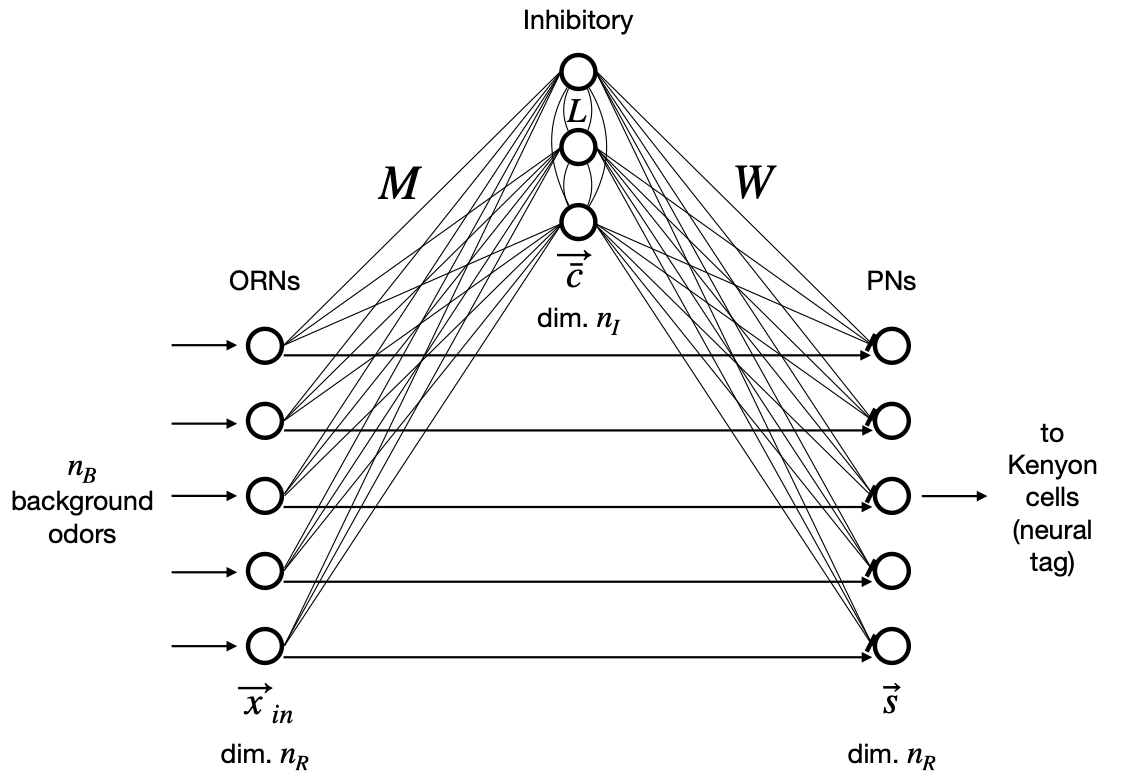
\includegraphics[width=0.8\textwidth]{figures/feedforward_inhibitory_network.pdf}
	\caption{Proposed olfactory habituation network model, where inhibitory neurons decompose the current background into components that are recombined to suppress the background ad its fluctuations. }
	\label{fig:inhibition_network}
\end{figure}

Second, the network has to learn inhibitory weights $W$ that can use the projections in the inhibitory neurons $\vec{\ovl{c}}$ to suppress the incoming background odor mixture. It turns out that local and Hebbian learning rules for the $W$ weights can be derived from a simple optimization problem, without regard to the details of how the projection weights $M$ and $L$ are learnt. We present these learning rules for $W$ synapses in this section; later on, they can be combined with IBCM neurons, PCA neurons, ICA neurons, or any other kind of inhibitory neurons. 

% Optimal W derivation. 
\subsection{Derivation of optimal inhibitory synaptic weights}
\label{subsect:optimal_inhib_weights}

% Cost function for W
\subsubsection{Cost function for $W$ optimization}
\label{subsubsect:cost_function}

During the learning phase (i.e. exposition to the background only), we want the inhibitory neurons to silence the activity of projection neurons in response to the varying input. Define $\vec{s}$ the vector of PN activities, with 

\beq
	\vec{s}= R(\vec{x}_{in} -  W\vec{\ovl{c}})   \quad ,
	\label{eq:pn_relu}
\eeq

where $R$ is an element-wise activation function (e.g., identity or ReLU), and $W\vec{\ovl{c}}$ is the output sent by the inhibitory neurons to projection neurons. Each column of $W$ is the vector $\vec{w}_j$ of synaptic weights leaving inhibitory neuron $j$ towards the different PNs in $\vec{s}$. 

We want the inhibitory weight matrix $W$ to minimize the norm of $\vec{s}$. This objective is encapsulated in the cost function

\beq
	C(W) = \frac12 \esper{\vec{s}^T \vec{s}} + \frac12 \frac{\beta}{\alpha} \esper{\vec{w}^T \vec{w}}
	\label{eq:cost_w}
\eeq

The first term ensures minimization of $\vec{s}$'s magnitude. The second term is a regularization ensuring $\vec{w}$ does not diverge when, for instance, $R$ is a ReLU function, such that large negative values of $\vec{w}$ would make $\vec{s}$ zero. In other words, the regularization ensures that the layer inhibits just enough the background and will still let through some of the new odor when it arrives. The parameter $\frac{\beta}{\alpha}$ controls the magnitude of this regularization (the choice of the form $\beta/\alpha$ will become clear below).

% Gradient calculation
\subsubsection{Gradient descent equations}
\label{subsubsect:gradient_descent}
We use gradient descent dynamics for the weights $\vec{w}_j$, 

\beq
	\frac{d \vec{w}_j}{dt} = - \alpha \vec{\nabla}_{\vec{w}_j} C(W)
	\label{eq:gradient_descent_w}
\eeq

so we need to compute the gradient of $C(W)$ with respect to each weight vector $\vec{w}_j$ (the $j$th column of $W$). The regularization term simply gives 
\beq
	\vec{\nabla}_{\vec{w}_j} \esper{\vec{w}^T \vec{w}} = 2 \esper{\vec{w}_j}   \,\,\, .
	\label{eq:gradient_regul}
\eeq
The $\vec{s}$ term gives 
\beq
	\vec{\nabla}_{\vec{w}_j} \esper{\vec{s}^T \vec{s}} = 2 \sum_k \esper{s^k \vec{\nabla}_{\vec{w}_j} s^k} \, \, \, .
	\label{eq:gradient_pn}
\eeq
We need to evaluate the derivative of $\vec{s} = R(\vec{x}_{in} - \sum_l \ovl{c}^l w^{kl})$, where $R$ is the PN activation function, for instance identity or ReLU. It is best worked out in index notation (Einstein summation of repeated indices applies except to $k$):

\begin{align}
	\vec{\nabla}_{\vec{w}_j} s^k & = \vec{\nabla}_{\vec{w}_j} R(x^k - w^k_l \ovl{c}^l w^{kl}) \nonumber \\
		&= - \hat{e}^i \frac{\partial}{\partial w^i_j} \left( w^k_l \ovl{c}^l \right) \frac{\partial R}{\partial s^k} \nonumber \\
		&= - R'(s^k) \hat{e}^i \delta_i^k \delta_l^j \ovl{c}^l \nonumber  \\
		&= -R'(s^k) \hat{e}^k \ovl{c}^j     \label{eq:gradient_calculation}
\end{align}

We will drop the averages and assume the rate $\alpha$ is small enough to effectively perform a time-averaging over the rapidly fluctuating inputs. We can finally combine equations \eqref{eq:gradient_regul}, \eqref{eq:gradient_pn}, and \eqref{eq:gradient_calculation} into equation \eqref{eq:gradient_descent_w} to obtain the optimal learning rule for the $\vec{w}_j$:

\beq
	\frac{d \vec{w}_j}{dt} = \alpha \ovl{c}^j \overrightarrow{sR'(s)} - \beta \vec{w}_j \quad ,
	\label{eq:learning_rule_w}
\eeq
where $\overrightarrow{s R'(s)}$ indicates that $R'$ is applied to $\vec{s}$ and multiplied to $\vec{s}$ element-wise. When $R$ is the identity function or a ReLu function, we can omit $R'(s)$: this is obvious for the identity case, while for the ReLU case, $s^k \underline{R'}(s^k) = s^k$, because $R'$ is the Heaviside step function ($1$ if $s^k > 0$, $0$ else) and $s^k$ in front of $R'$ is already zero anyways when $R'$ itself would be null. Note that $\alpha$ and $\beta$ are the learning rates of the $W$ synapses; usually, one takes $\beta < \alpha$ to ensure that $\vec{s}$ minimization is the dominant term of the cost function, and that background inhibition is efficient. 

The equation can be recast in matrix form for the whole $W$ using the outer product of $\vec{\ovl{c}}$ with $\vec{s}$ (we drop $R'$ for simplicity):

\beq
	\frac{dW}{dt} = \alpha {\vec{s}} \, \vec{\ovl{c}}^T - \beta W
	\label{eq:learning_rule_w_matrix}
\eeq

\subsection{Discussion of the inhibitory weights learning rule}
\label{subsect:discussion_w}

In component notation, equation \ref{eq:learning_rule_w} becomes
\beq
	\frac{d w^i_j}{dt} = \alpha \ovl{c}^j s^i R'(s^i) - \beta w^i_j \quad 
	\label{eq:learning_rule_w_components}
\eeq
This rule is seen to be completely local: $w^i_j$ only depends on the activities $\ovl{c}^i$ and $s^j$ of the neurons at its endpoints. It is also Hebbian, since the reinforcement of the connection is proportional to the product of those two activities. This makes such an inhibitory network biologically plausible. 

What exactly is being learnt with those weights $W$? The cost function introduced above aims, when $\beta = 0$, to minimize the norm of $\vec{s}$, that is (using $R = $ identity function for simplicity), to minimize $\| \vec{x} - W \vec{\ovl{c}} \|^2 = \| \vec{x} - W LM \vec{x}| \|^2$ with respect to $W$. For given $LM$ (learnt from IBCM, PCA, ICA, etc.), we know from linear algebra that the Moore-Penrose pseudo-inverse $(LM)^+$ minimizes this cost function{\protect
\footnote{Given a singular value decomposition (SVD) of a matrix $A = U \Sigma V^T$, the Moore-Penrose pseudo-inverse of $A$ is $A^+ = V \Sigma^+ U^T$, where $\Sigma^+$ has the inverse of the singular values on its diagonal. The pseudo-inverse solution to the minimization problem can actually be derived using SVD.}}. 
Therefore, the learning rule \eqref{eq:learning_rule_w} yields the Moore-Penrose pseudo-inverse -- or rather, an approximation of it, because of the regularization term. 


Therefore, the proposed network performs feedforward inhibition by learning approximately a projector on the background subspace, $P = \frac{\alpha}{\alpha + \beta}(LM)^+ (LM)$, and subtracting the input projection on that subspace from the full input: $\vec{s} = \vec{x} - P\vec{x}$. This leaves in $\vec{s}$ the input component that is orthogonal to the background (because of the regularization term, part of the orthogonal component persists in practice). In this sense, the network operates as an autoencoder with one hidden layer, learning a latent space to encode the olfactory background in the inhibitory neurons layer with matrices $LM$, and decoding them back to the full space with the weights $W$ to subtract that projection from the input, in $\vec{s} = \vec{x} - WLM \vec{x}$. 

The performance of this feedforward inhibition scheme will depend on the projections learnt via the $L$ and $M$ synaptic weights. We now discuss different models in the following sections, chiefly the IBCM model. 
